\chapter{Graph Construction}


\section{Similarity-based methods}
\subsection{Spearman}
\label{subsec:spearman_graphs}

\subsubsection{Node and Edge Distribution}
\label{subsubsec:spearman_node_edge_distribution}

Spearman correlation was used as a similarity criterion to construct the dynamic product graphs. In this setting, the objective is not to connect products with similar absolute sales volumes, but rather products whose demand evolves with a similar relative ordering within each temporal window. This is particularly relevant in retail demand forecasting, since two products may operate at very different sales scales while still exhibiting comparable short-term demand movements.
\begin{figure}
    \centering
    
\includegraphics[width=0.5\linewidth]{figures/hist_focal_vs_full_spearman_similarity_W30_S1_top1pct.png}
    \caption{Enter Caption}
    \label{fig:placeholder}
\end{figure}

\paragraph{Threshold Selection}

To guide threshold selection, the full pairwise Spearman similarity distribution 
was computed across all sliding windows, comparing each of the 61 benchmark 
products against the complete product catalogue. The resulting distribution, 
shown in Figure~\ref{fig:spearman_focal_vs_full_top1pct}, reveals that the vast 
majority of product pairs exhibit relatively low similarity: the bulk of the mass 
is concentrated below 0.4, indicating that most products do not share a 
meaningfully correlated demand pattern within any given 30-day window. The 
distribution is heavily right-skewed, with a long but thin tail extending towards 
higher similarity values.

This tail corresponds to the minority of pairs that exhibit genuine monotonic 
co-movement and thus represent candidates for graph edges. The top 1\% of all 
pairwise similarities begins at approximately $\tau = 0.574$, which established 
the lower bound for the threshold search. Values below this point fall within the 
dense body of the distribution, where most pairs are weakly correlated, and 
including them would introduce noise into the neighbourhood structure while 
substantially increasing computational cost. Within the tail, three threshold 
values were selected for evaluation: $\tau \in \{0.60,\, 0.65,\, 0.70\}$. 
Setting $\tau = 0.60$ retains the broadest set of relationships, producing 
graphs with a mean neighbourhood of approximately 5--10 nodes per product, 
which provides richer relational context at the cost of including weaker 
associations. Raising the threshold to $\tau = 0.65$ yields sparser graphs 
with 2--4 mean neighbours, while $\tau = 0.70$ produces very sparse graphs 
with only 1--2 mean neighbours, retaining exclusively the strongest monotonic 
co-movement signals.

\paragraph{Effect of Threshold on Graph Density}

Figure~\ref{fig:mean_nodes_th070}--\ref{fig:mean_nodes_th060} show the mean 
number of nodes per sliding window across the 61 benchmark products for 
$\tau \in \{0.70,\, 0.65,\, 0.60\}$. Several consistent patterns emerge 
across all configurations.

\textbf{Temporal structure.} Graph density is far from uniform over time. 
Two pronounced density spikes are visible regardless of threshold: one 
concentrated around late February 2021 — the earliest windows in the 
training set — and a second, sharper spike around Thanksgiving--Christmas 
2021 (late November to early January 2022). Outside these episodes, the 
mean node count stabilises at a low baseline, indicating that strong 
monotonic co-movement among products is the exception rather than the rule 
during ordinary trading periods.

\textbf{Impact of threshold.} The threshold exerts a strong and predictable 
influence on graph density. At $\tau = 0.70$, the peak mean reaches 14.1 
nodes (22/02/2021) and the typical off-peak mean is approximately 1--2 
neighbours per product, producing very sparse graphs. Lowering the threshold 
to $\tau = 0.65$ raises the peak to 29.4 nodes and the off-peak baseline 
to roughly 2--4 neighbours. At $\tau = 0.60$ the peak surges to 56.9 nodes 
and the baseline climbs to approximately 5--10 neighbours, offering a denser 
neighbourhood representation that may provide the GNN with richer relational 
context during non-seasonal periods.

\textbf{Dispersion.} The shaded $\pm 1$ standard deviation band widens 
considerably as $\tau$ decreases, revealing growing heterogeneity across 
products: at lower thresholds, certain products accumulate a large number 
of neighbours while others remain isolated, which may bias the message-passing 
aggregation towards better-connected products.

\textbf{Selection rationale.} All three thresholds $\tau \in \{0.60,\, 0.65,\, 0.70\}$ 
were retained for experimental evaluation. Each represents a distinct 
operating regime — dense, moderate, and sparse — allowing the downstream 
forecasting results to determine empirically which level of graph connectivity 
is most beneficial for the GNN model.

Table~\ref{tab:spearman_threshold_density} summarises the key density 
statistics for each threshold.

\begin{table}[htbp]
\centering
\caption{Graph density statistics as a function of the Spearman similarity 
threshold $\tau$, computed over 30-day sliding windows with step $s = 1$ day 
across the 61 benchmark products. Mean neighbours refers to the mean number of 
nodes adjacent to the central product, averaged across all products and 
all non-peak windows. Peak neighbours is the maximum mean node count observed 
at any single window.}
\label{tab:spearman_threshold_density}
\begin{tabular}{ccccc}
\toprule
\textbf{Threshold} $\tau$ 
    & \textbf{Off-peak mean neighbours} 
    & \textbf{Peak mean neighbours} 
    & \textbf{Peak date} 
    & \textbf{Graph regime} \\
\midrule
0.70 & $\approx 1$--$2$ & 14.1 & 22/02/2021 & Very sparse \\
0.65 & $\approx 2$--$4$ & 29.4 & 24/02/2021 & Sparse      \\
0.60 & $\approx 5$--$10$ & 56.9 & 24/02/2021 & Moderately dense \\
\bottomrule
\end{tabular}
\end{table}
\begin{figure}[htbp]
    \centering
    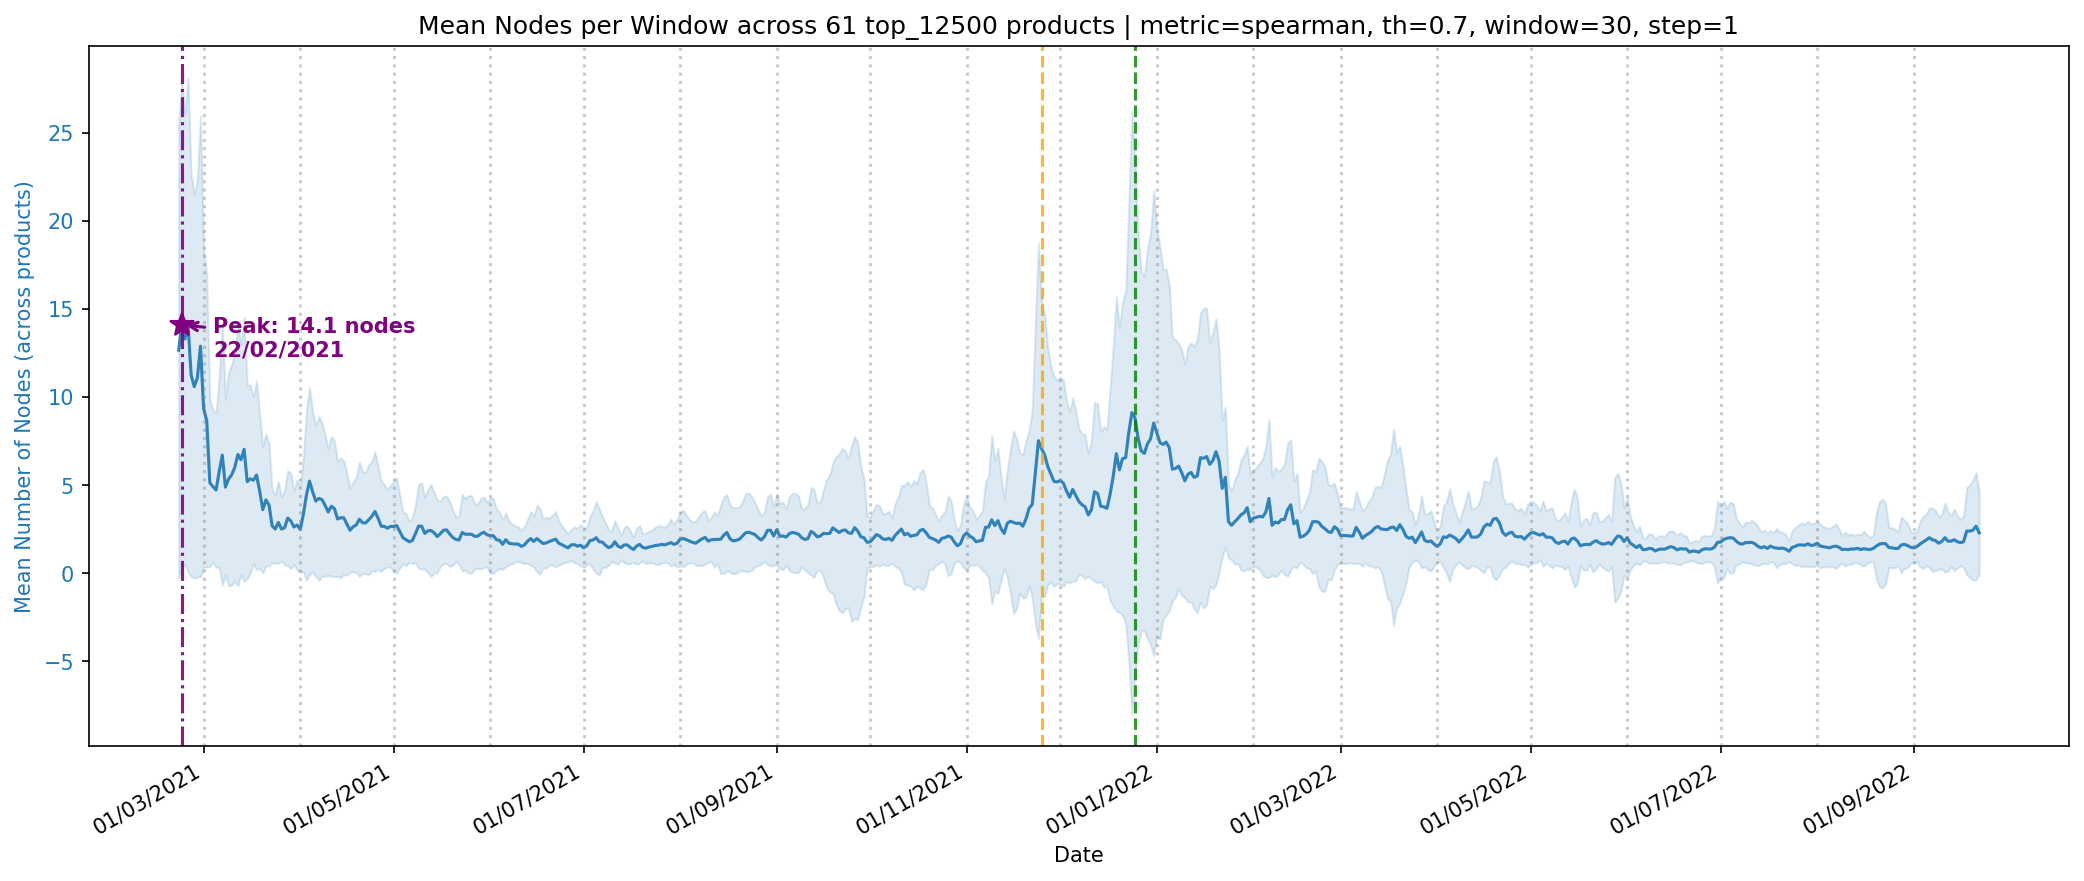
\includegraphics[width=\textwidth]{figures/mean_nodes_per_window.png}
    \caption{Mean number of graph nodes per sliding window across the 61 benchmark products, computed using Spearman similarity with threshold $\tau = 0.75$, window size $W = 30$ days and step $s = 1$ day. The shaded region represents $\pm 1$ standard deviation across products. Vertical dashed lines mark Christmas (25 December, \textcolor{green}{green}), Thanksgiving (fourth Thursday of November, \textcolor{orange}{orange}), and month boundaries (\textcolor{gray}{gray}). The purple marker indicates the window with the highest mean node count.}
    \label{fig:mean_nodes_per_window_spearman_th075}
\end{figure}

\subsection{Kendall}
\label{subsec:kendall_graphs}

\subsubsection{Node and Edge Distribution}
\label{subsubsec:kendall_node_edge_distribution}

Kendall correlation was also considered as a similarity criterion for the construction of the dynamic product graphs. Similarly to Spearman correlation, Kendall is based on the relative ordering of the observations rather than on their absolute magnitude. However, instead of correlating ranked values directly, Kendall evaluates the degree of concordance between pairs of observations. In this context, two products are considered similar when their demand variations preserve a consistent ordering within the same temporal window.

This makes Kendall a stricter and more conservative measure of monotonic association. While Spearman captures whether two series tend to move according to a similar ranked pattern, Kendall requires a stronger pairwise agreement between the temporal observations. As a result, Kendall-based graphs are expected to be more selective, especially when demand series contain short-term noise, local irregularities, or intermittent sales behaviour.

For each target product, Kendall similarities were computed over sliding windows of 15 days. In each window, the target product was compared with all active candidate products, and an edge was created whenever the Kendall similarity exceeded the selected threshold. Therefore, as in the Spearman case, the resulting graph sequence is dynamic: the number of neighbouring nodes and the number of edges may vary from one window to another according to the strength of the local product relationships.

\begin{figure}[h]
    \centering
    
\includegraphics[width=0.5\linewidth]{kendall_edge_distribution.png}
    \caption{Enter Caption}
    \label{fig:placeholder}
\end{figure}
The temporal evolution of nodes and edges provides an indication of how restrictive the Kendall criterion is across the demand horizon. Since Kendall is based on concordant and discordant pairs, the resulting graphs tend to retain only relationships where the relative demand ordering is highly consistent. Consequently, windows with few nodes and edges indicate periods where the target product does not share a sufficiently stable monotonic pattern with many other products. In contrast, occasional increases in graph density suggest periods of stronger synchronization between products, which may be associated with seasonal demand effects, promotional events, or broader calendar-driven consumption patterns.

\begin{figure}
    \centering
    
\includegraphics[width=0.5\linewidth]{kendall_node_and_edge_distribution.png}
    \caption{Enter Caption}
    \label{fig:placeholder}
\end{figure}

Compared with Spearman, Kendall may produce sparser graphs for equivalent threshold levels, because it penalizes local inconsistencies more strongly. This behaviour is useful from a graph construction perspective because it allows the model to focus on more robust monotonic relationships, reducing the probability of including unstable or incidental co-movements. However, excessive sparsity may also limit the amount of relational information available to the forecasting model, making threshold selection particularly important.

\paragraph{Threshold Selection and Percentile Matching}

The threshold selection for Kendall follows the same principle adopted for Spearman: different cutoff values are evaluated to control the trade-off between graph density and relational selectivity. However, applying the exact numerical thresholds used for Spearman directly to Kendall is methodologically unsound due to the inherent scaling differences between the two metrics. 

Empirically and theoretically, Kendall correlation values are systematically lower than Spearman correlation values ($|\tau| < |\rho|$) for any dataset that is not perfectly monotonic. This systematic compression arises from two distinct mathematical and domain-specific factors:

\begin{enumerate}
    \item \textbf{Concordance versus Distance:} Spearman calculates a standard Pearson correlation over the ranks, meaning it measures the absolute mathematical distance between ranks and heavily penalizes large rank discrepancies. In contrast, Kendall strictly evaluates the ratio of concordant pairs ($C$) to discordant pairs ($D$), entirely ignoring the magnitude of the distance between them. Because Kendall relies on binary disagreements rather than continuous distance, it is mathematically more conservative.
    \item \textbf{The Ties Penalty in Retail Demand:} Retail time series, particularly over short 30-day sliding windows, are highly sparse and contain numerous days with zero sales. These identical values create "ties" in the ranking process. Kendall's Tau-b specifically incorporates a mathematical penalty for ties in its denominator. Consequently, the flat periods typical of intermittent retail demand heavily depress the Kendall similarity scores, whereas Spearman often artificially inflates them under the same conditions.
\end{enumerate}

To ensure topological consistency—meaning the Kendall graphs maintain an equivalent degree of sparsity and edge density to the Spearman graphs—thresholds must be aligned via percentile matching rather than raw numerical equivalence. Specifically, the threshold calibration was guided by isolating the top 1\% of pairwise connections between the 61 benchmark products and the full product catalogue (comprising over 500,000 candidate observations). By analyzing the extreme right tail of this global similarity distribution, Kendall thresholds were selected to filter the exact same proportion of the most highly correlated edges as their Spearman counterparts.

Based on the empirical distribution percentiles, the candidate Kendall thresholds evaluated in this study are defined as:

\begin{equation}
    \tau \in \{0.46, 0.50, 0.54\}
\end{equation}

These values correspond directly to the graph densities generated by the Spearman thresholds of 0.60, 0.65, and 0.70, respectively. For instance, a Kendall threshold of 0.54 and a Spearman threshold of 0.70 both isolate approximately the top 10\% to 15\% of the most strongly correlated product pairs. 

For each value of $\tau$, an edge is created only when the Kendall similarity is greater than or equal to the selected threshold. Lower values of $\tau$ (e.g., 0.46) favour broader neighbourhoods and allow the model to exploit more relational context, although with a higher risk of including weaker dependencies. Higher values of $\tau$ (e.g., 0.54) enforce a stricter graph structure, emphasizing only products with highly stable monotonic agreement.

\begin{figure}[ht]
    \centering
    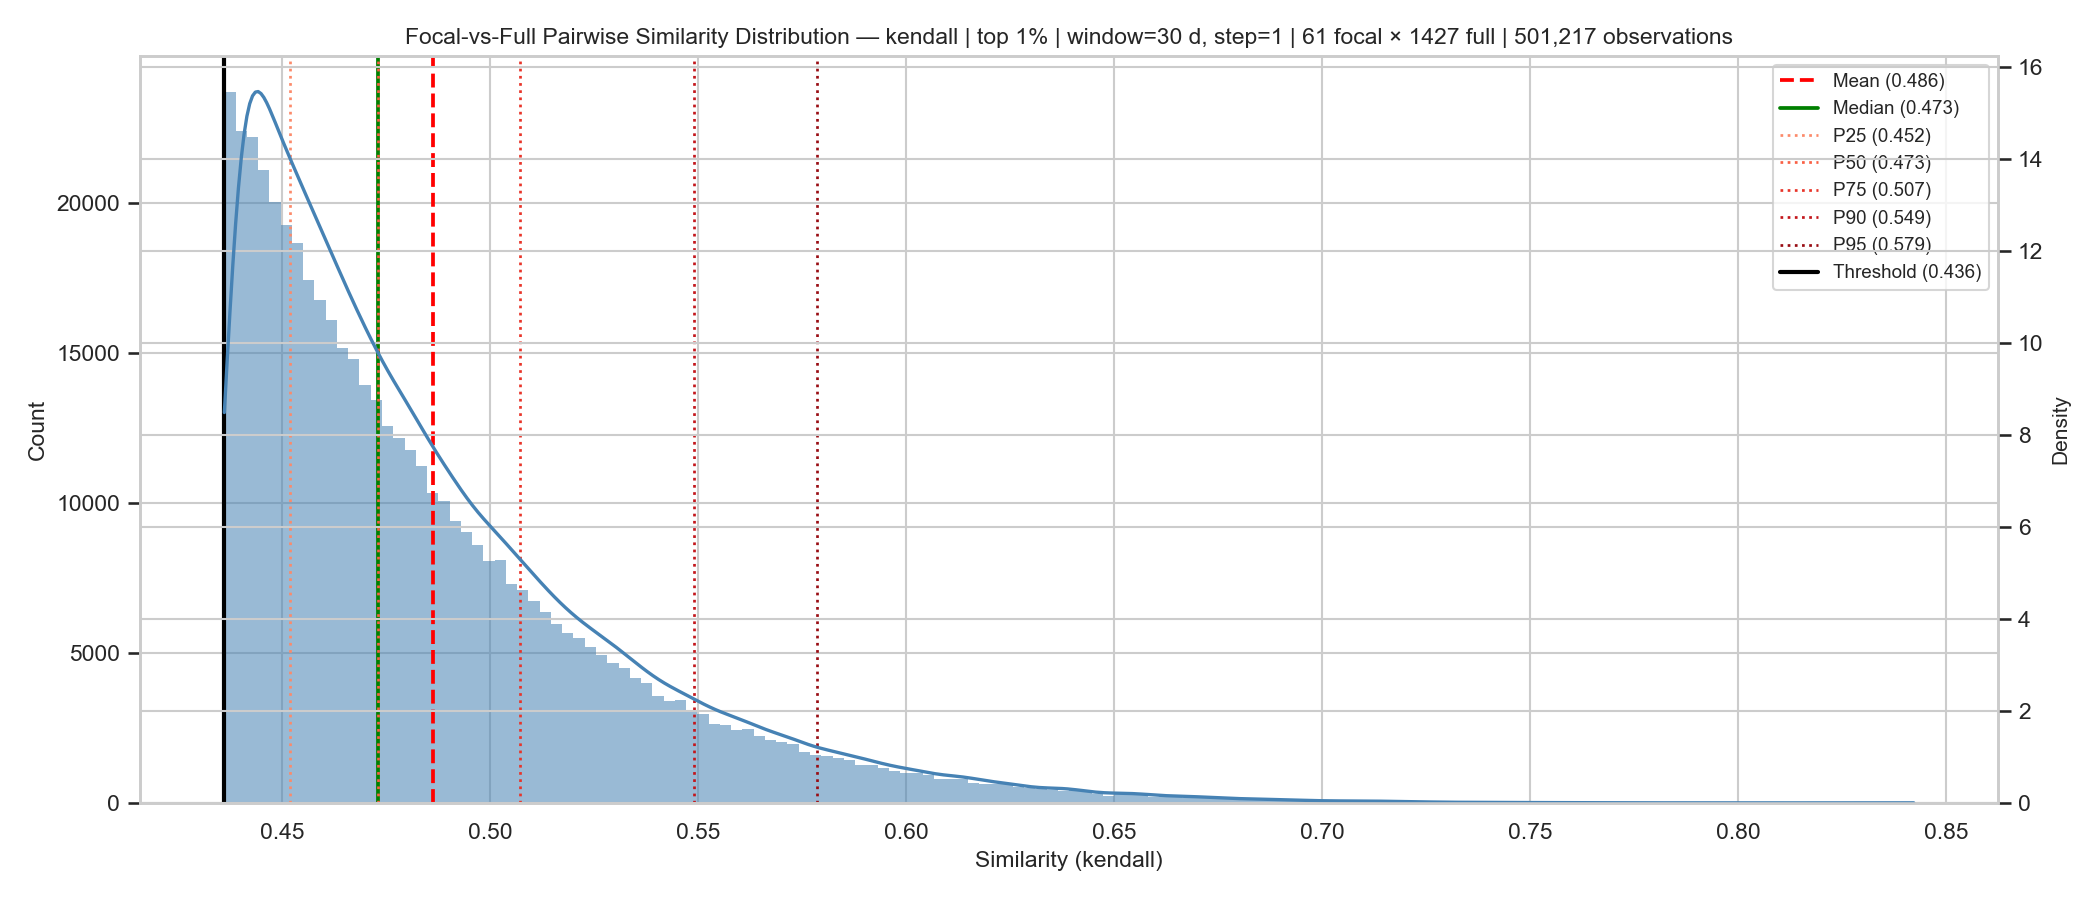
\includegraphics[width=0.8\linewidth]{figures/kendall_top1.png}
    \caption{Distribution of pairwise Kendall similarities demonstrating the percentile-matched threshold cutoff.}
    \label{fig:kendall_percentile_distribution}
\end{figure}

Thus, the Kendall threshold selection procedure provides a controlled way to evaluate whether the forecasting model benefits from conservative relational structures. If performance improves under higher thresholds, this suggests that the model relies on a smaller set of highly reliable neighbours. Conversely, if intermediate thresholds perform better, it indicates that a broader product context remains useful even when the monotonic agreement is strictly evaluated.
\section{Distance-based measurements}

\subsection{Data Preprocessing}

Before computing any distance-based similarity between time series, a critical preprocessing step must be addressed: the heterogeneity of sales volumes across products. In a retail setting, it is common for different stock-keeping units (SKUs) to exhibit dramatically different absolute scales — a high-volume staple product may register hundreds of units sold per day, while a niche or seasonal item may sell only a handful of units over the same period. If raw sales values are fed directly into a distance function such as the Euclidean distance, the resulting metric will be dominated by amplitude differences rather than by the underlying temporal pattern or trend structure that is relevant for graph construction.

To eliminate this scale bias, a per-item \textit{Z-score normalisation} is applied prior to computing pairwise distances. Formally, for each item $i$ with training-set time series $\mathbf{x}_i^{\text{train}} = (x_{i,1}, \ldots, x_{i,T_{\text{train}}})$, the item-specific mean $\mu_i$ and standard deviation $\sigma_i$ are estimated exclusively on the training window:

\begin{equation}
    \mu_i = \frac{1}{T_{\text{train}}} \sum_{t=1}^{T_{\text{train}}} x_{i,t}, \qquad
    \sigma_i = \sqrt{\frac{1}{T_{\text{train}}} \sum_{t=1}^{T_{\text{train}}} \left(x_{i,t} - \mu_i\right)^2}.
\end{equation}

The full time series (including validation and test periods) is then transformed as

\begin{equation}
    \tilde{x}_{i,t} = \frac{x_{i,t} - \mu_i}{\sigma_i + \varepsilon},
\end{equation}

where $\varepsilon$ is a small constant added for numerical stability. This ensures that all items are expressed in units of standard deviations from their own training mean, making the resulting series zero-centred with unit variance during the training period.

An important aspect of this procedure is that the scaler is \textit{fitted only on the training split} and then applied to the entire time axis. This discipline prevents any leakage of future statistical information into the graph construction process, which is critical given that the graphs are later used as inputs to a forecasting model. The normalised series $\tilde{\mathbf{x}}_i$ are then used in all subsequent distance computations.

\subsection{Euclidean Distance}

After normalisation, the Euclidean distance between two time series segments of length $w$ (corresponding to a sliding window) is defined as

\begin{equation}
    d_{\text{Euc}}(\mathbf{a}, \mathbf{b}) = \left\| \mathbf{a} - \mathbf{b} \right\|_2 = \sqrt{\sum_{k=1}^{w} \left(a_k - b_k\right)^2}.
\end{equation}

Because both series have been standardised to comparable scales, this quantity now reflects \textit{shape dissimilarity} rather than amplitude magnitude. Two products with similar seasonal patterns but vastly different absolute volumes will yield a small Euclidean distance after normalisation, whereas products with divergent temporal dynamics will yield a large one.



